\documentclass{article} % This command is used to set the type of document you are working on such as an article, book, or presenation

\usepackage{geometry} % This package allows the editing of the page layout
\usepackage{amsmath}  % This package allows the use of a large range of mathematical formula, commands, and symbols
\usepackage{graphicx}  % This package allows the importing of images
\usepackage{soul}
\usepackage{amsfonts}
\usepackage{dirtytalk}
\usepackage{tabto}
\usepackage{xcolor,colortbl, amssymb}
\usepackage{forest, tikz}

% https://www.messletters.com/en/big-text/

\newcommand{\question}[2][]{\begin{flushleft}
        \textbf{Problem #1}: \textit{#2}

\end{flushleft}}

\definecolor{Green}{rgb}{0, 1, 0}
\definecolor{Pink}{rgb}{1, .753, .796}

\newcommand{\sol}{\textbf{Solution}:} %Use if you want a boldface solution line
%\newcommand\tab[1][0.4cm]{\hspace*{#1}}
\newcommand{\maketitletwo}[2][]{\begin{center}
        \Large{\textbf{Homework #1}
            
            CMPSC 465} % Name of course here
        \vspace{5pt}
        
        \normalsize{Kinner Parikh  % Your name here
        
        \today}        % Change to due date if preferred
        \vspace{40pt}


        \newpage
        
\end{center}}
\begin{document}
    \maketitletwo[1]  % Optional argument is assignment number
    %Keep a blank space between maketitletwo and \question[1]

    \question[1]{}
    \begin{center}
        
        I did not work in a group
    
        I did not consult without anyone my group member
    
        I did not consult any non-class materials
    \end{center}
    
    \newpage

    \question[2]{DFS Basics}

    a) $A,\ B,\ D,\ E,\ G,\ F,\ C,\ H,\ I$

    \vspace{5pt}

    b) $A(1, 12), B(2, 11), D(3, 6), E(4, 5), G(7, 10), F(8, 9), C(13, 18), H(14, 17), I(15, 16)$

    \vspace{5pt}

    c) Tree Edges: \hspace{16pt}\{$(A, B), (B, D), (D, E), (B, G), (G, F), (C, H), (H, I)$\}

    \hspace{12pt}Back Edges: \hspace{14pt}\{$(E, D)$\}

    \hspace{12pt}Forward Edges: \{$(A, E), (C, I)$\}

    \hspace{12pt}Cross Edges: \hspace{12pt}\{$(G, D)$\}

    \newpage

    \question[3]{Pre and Post Processing}

    \newpage

    \question[4]{Linearization Basics}

    a) (pre, post)
    
    \vspace{3pt}

    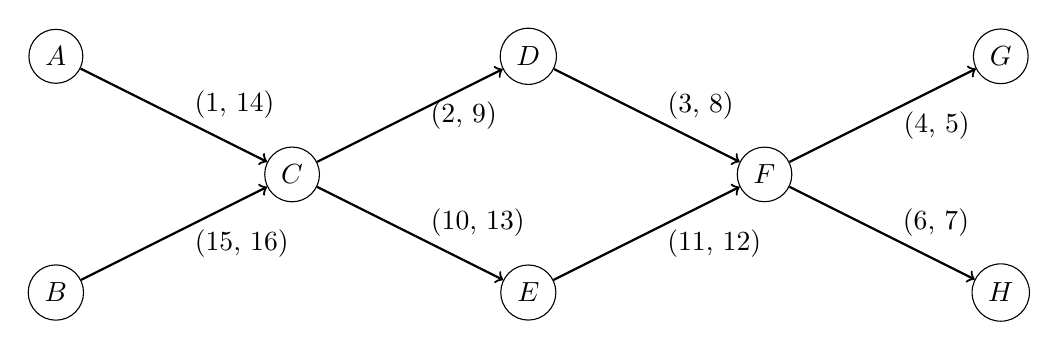
\begin{tikzpicture}[scale=1.5,auto=center]

        \node[circle, draw] (a) at (1, 4-1) {$A$};
        \node[circle, draw] (b) at (1, 2-1) {$B$};
        \node[circle, draw] (c) at (3, 3-1) {$C$};
        \node[circle, draw] (d) at (5, 4-1) {$D$};
        \node[circle, draw] (e) at (5, 2-1) {$E$};
        \node[circle, draw] (f) at (7, 3-1) {$F$};
        \node[circle, draw] (g) at (9, 4-1) {$G$};
        \node[circle, draw] (h) at (9, 2-1) {$H$};

        \path[->,draw,thick]
        (a) edge node[label = right:\text{(1, 14)}, above]{} (c)
        (b) edge node[label = right:\text{(15, 16)}, below]{} (c)
        (c) edge node[label = right:\text{(2, 9)}]{} (d)
        (c) edge node[label = right:\text{(10, 13)}, above]{} (e)
        (d) edge node[label = right:\text{(3, 8)}, above]{} (f)
        (e) edge node[label = right:\text{(11, 12)}, below]{} (f)
        (f) edge node[label = right:\text{(4, 5)}, below]{} (g)
        (f) edge node[label = right:\text{(6, 7)}, above]{} (h)
        ;
        
    \end{tikzpicture}

    \vspace{4pt}

    b) Source Nodes: $A, B$

    \hspace{10pt} Sink Nodes: $G, H$

    \vspace{4pt}

    c) 

    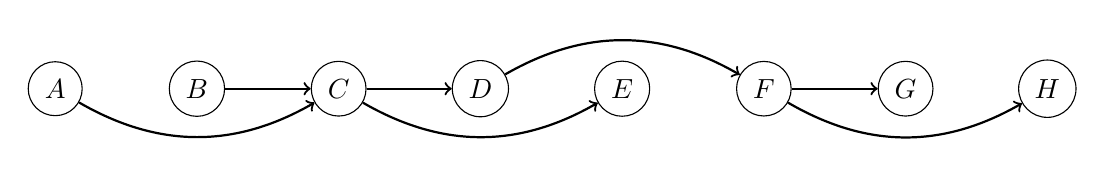
\begin{tikzpicture}[scale=0.9,auto=center]
        \node[circle, draw] (a) at (0, 0) {$A$};
        \node[circle, draw] (b) at (2, 0) {$B$};
        \node[circle, draw] (c) at (4, 0) {$C$};
        \node[circle, draw] (d) at (6, 0) {$D$};
        \node[circle, draw] (e) at (8, 0) {$E$};
        \node[circle, draw] (f) at (10, 0) {$F$};
        \node[circle, draw] (g) at (12, 0) {$G$};
        \node[circle, draw] (h) at (14, 0) {$H$};


        \draw[->, thick] (a) to[bend right] (c);
        \draw[->, thick] (b) to (c);
        \draw[->, thick] (c) to (d);
        \draw[->, thick] (c) to[bend right] (e);
        \draw[->, thick] (d) to[bend left] (f);
        \draw[->, thick] (f) to (g);
        \draw[->, thick] (f) to[bend right] (h);
        
    \end{tikzpicture}

    d) This graph will have 8 total linearizations 
\end{document}
